\documentclass[a5paper]{article}
\usepackage[dutch]{babel}
\usepackage{tikz}
\usepackage[margin=0.5cm]{geometry}
\usepackage{amsmath, amssymb, amsfonts}
\usepackage{graphicx}
\usepackage{enumitem}
\usepackage{multicol}
\usepackage{titlesec}
\usepackage{hyperref}
\usepackage{adjustbox}

\usepackage{array}  % For better table alignment
\usepackage{float}  % To control the placement of the table

% Adjust spacing for sections and subsections
\titlespacing*{\section}{0pt}{*1}{0pt} % Reduce spacing after section heading
\titlespacing*{\subsection}{0pt}{*0.5}{0pt} % Reduce spacing after subsection heading


% Adjust table spacing
\setlength{\textfloatsep}{0pt} % Reduce spacing before and after tables

\begin{document}

\title{Formularium Wiskunde}
\author{Ian Claesen}
\date{\today}
\maketitle

\scriptsize
\tableofcontents

\newpage
\normalsize

\section{Algebra}
\subsection{Volgorde van Bewerking}
Haakjes wegwerken, machtsverheffen, worteltrekken, vermenigvuldigen en delen, optellen en aftrekken.

\subsection{Absolute Waarde}
De absolute waarde van een getal $a$ wordt genoteerd als $|a|$ en is altijd positief.
\[
|a| = \begin{cases} 
a & \text{if } a \geq 0 \\
-a & \text{if } a < 0 
\end{cases}\]

\section{Machten en wortels}
\subsection{Machten met Gehele Exponenten}
\renewcommand{\arraystretch}{1.5} % Adjust row height

\[
\begin{array}{|c|c|}
\hline
\begin{array}{l}
\forall a \in ,\forall n \in {\mathbb{N}_0}:{a^n} = \underbrace {a.a.\;...\;.a}_{n\;factoren}\\
\forall a \in {\mathbb{R}}:\;{a^1} = \;a\\
\forall a \in {\mathbb{R}_0}:\;{a^0} = \;1\\
\forall a \in {\mathbb{R}_0},\forall n \in {\mathbb{N}}:\;{a^{ - n}} = \;\frac{1}{{{a^n}}}
\end{array} & \begin{array}{l}
\forall a,b \in {\mathbb{R}_0},\forall m,n \in {\mathbb{Z}}:{a^m} \cdot {a^n} = {a^{m + n}}\\
\frac{{{a^m}}}{{{a^n}}} = {a^{m - n}}\\
{({a^m})^n} = {a^{mn}}\\
{(a.b)^n} = {a^n} \cdot {b^n}\\
{\left( {\frac{a}{b}} \right)^n} = \frac{{{a^n}}}{{{b^n}}}\\
{\left( {\frac{a}{b}} \right)^{ - n}} = {\left( {\frac{b}{a}} \right)^n}
\end{array} \\ 
\hline
\end{array}
\]

\subsection{Vierkantswortel in $\mathbb{R}$}

\[
\begin{array}{|c|c|}
\hline
\begin{array}{l}
\forall a\in\mathbb{R}^+,\forall b\in\mathbb{R}:\\
 b=\sqrt a\Leftrightarrow b^2=a\,\land\,(b\geq0)\\
\forall a,b\in\mathbb{R}^+:\\
\hspace{1cm}\sqrt{a^2}=a\\
\hspace{1cm}\left(\sqrt a\right)^2=a\\
\hspace{1cm}\sqrt{ab} = \sqrt{a} \cdot \sqrt{b}.\\
\hspace{1cm}\sqrt{\frac{a}{b}} = \frac{\sqrt{a}}{\sqrt{b}} \land b \neq 0\\
\end{array} & \begin{array}{l}
\forall a\in\mathbb{R}:\\
\sqrt{a^2} = \left|a\right| \implies 
\begin{cases} 
    \sqrt{a^2} = a & \text{als } a \geq 0, \\ 
    \sqrt{a^2} = -a & \text{als } a \leq 0.
\end{cases}
\end{array} \\ 
\hline
\end{array}
\]

\subsection{N-de machtswortel in $\mathbb{R}$}
\[
\begin{array}{|c|c|}
\hline
\begin{array}{l}
n\,\,even\Rightarrow\sqrt[n]{a^n}=\left|a\right|\rightarrow\left\{\begin{matrix}\sqrt[n]{a^n}=a&\land\, a\geq0\\\sqrt[n]{a^n}=-a&\land\, a\le0\\\end{matrix}\right.\,\\
n\,\, oneven\Rightarrow\sqrt[n]{a^n}=a
\end{array} & \begin{array}{l}
\forall a,b\in\mathbb{R}_0^+,\forall m,n\in\mathbb{N}_0:\\
\sqrt[n]{a^n}=a\\
\left(\sqrt[n]{a}\right)^n=a\\
\sqrt[n]{ab}=\sqrt[n]{a}.\sqrt[n]{b}\\
\sqrt[n]{\frac{a}{b}}=\frac{\sqrt[n]{a}}{\sqrt[n]{b}}\\
\sqrt[m]{\sqrt[n]{a}}=\sqrt[m.n]{a}
\end{array} \\ 
\hline
\end{array}
\]

\newpage

\subsection{$\frac{m}{n}$-de machtswortel in $\mathbb{R}$ }
\[
\begin{array}{|c|c|}
\hline
\begin{array}{l}
\forall a\in\mathbb{R}_0^+,\forall m\in\mathbb{Z},\forall n\in\mathbb{N}_0:a^\frac{m}{n}=\sqrt[n]{a^m}
\end{array} & \begin{array}{l}
\forall a,b\in\mathbb{R}_0^+,\forall m,n\in\mathbb{Q}:\\
a^m.a^n=a^{m+n}\\
\frac{a^m}{a^n}=a^{m-n}\\
\left(a^m\right)^n=a^{m.n}\\
\left(a.b\right)^m=a^m.b^m\\
\left(\frac{a}{b}\right)^m=\frac{a^m}{b^m}
\end{array} \\ 
\hline
\end{array}
\]

\section{Veeltermen}
\subsection{Vierkantsvergelijking}
$Een\:vierkantsvergelijking\:is\:van\:de\:vorm:\:ax^2 + bx + c = 0\:,\:met\:D=b^2 - 4ac $

\renewcommand{\arraystretch}{1.5} % Adjust row height
\[
\begin{array}{|c|c|}
\hline
x\in{\displaystyle \mathbb {R} } & x\in{\displaystyle \mathbb {C} } \\ 
\hline
x_{1,2} = \frac{-b \pm \sqrt{D}}{2a} \quad  & x_{1,2} = \frac{-b \pm i\sqrt{-D}}{2a} \quad \\ 
\hline
P = \frac{c}{a} = x_1 \cdot x_2\:,\:S = -\frac{b}{a} = x_1 + x_2 &  \\ 
\hline
ax^2 + bx + c = a(x - x_1)(x - x_2) = a(x^2 - Sx + P) & \\
\hline
\end{array}
\]

\subsection{Merkwaardige Producten en Ontbinding in Factoren}
\[
\begin{array}{|l|l|}
\hline
(a\pm b)^2 = a^2 \pm 2ab + b^2 \\ 
\hline
{\left( {a \pm b} \right)^3} = {a^3} \pm 3{a^2}b + 3a{b^2} \pm {b^3} \\
\hline
{\left( {a + b} \right)^n} = {a^n} + C_n^1{a^{n - 1}}b + C_n^2{a^{n - 2}}{b^2} + ... + C_n^{n - 1}{a^2}{b^{n - 1}} + {b^n}\quad  \wedge \quad C_n^p = \frac{{n!}}{{\left( {n - p} \right)!p!}} \\
\hline
{a^2} - {b^2} = \left( {a + b} \right)\left( {a - b} \right) \\
\hline
{a^3} - {b^3} = \left( {a - b} \right)\left( {{a^2} + ab + {b^2}} \right) \\
\hline
{a^n} - {b^n} = \left( {a - b} \right)\left( {{a^{n - 1}} + {a^{n - 2}}b + {a^{n - 3}}{b^2} + ... + a{b^{n - 2}} + {b^{n - 1}}} \right) \\
\hline
{a^3} + {b^3} = \left( {a + b} \right)\left( {{a^2} - ab + {b^2}} \right) \\
\hline
{a^{2n + 1}} + {b^{2n + 1}} = \left( {a + b} \right)\left( {{a^{2n}} - {a^{2n - 1}}b + {a^{2n - 2}}{b^2} - {a^{2n - 3}}{b^3} + ... - a{b^{2n - 1}} + {b^{2n}}} \right) \\
\hline
\end{array}
\]

\newpage

\subsection{Euclidische Deling}
We gaan de derdegraadsveelterm $2x^3 + 3x^2 - 4x + 5$ delen door de eerstegraadsveelterm $x + 2$ met behulp van de praktische werkwijze van lange deling.

\[
\begin{array}{r|l}
   2x^3 + 3x^2 - 4x + 5 & x + 2 \\
  \hline
  -2x^3 - 4x^2 + 0x + 0 & 2x^2 \\
  \hline
        - 1x^2 - 4x + 5 & \\
        + 1x^2 + 2x + 0 & -x \\
  \hline
                -2x + 5 & \\
                 2x + 4 & -2 \\
  \hline
  9 & 
\end{array}
\]

We kunnen de deling als volgt uitdrukken:
\[
2x^3 + 3x^2 - 4x + 5 = (x + 2)(2x^2 - x - 2) + 9
\]

De rest is $25$, wat een graad heeft die kleiner is dan de graad van de deler $x + 2$.


\subsection{Schema van Horner}
\[
\frac{(3x^3-5x^2+10x-52)}{(x-2)}
\]

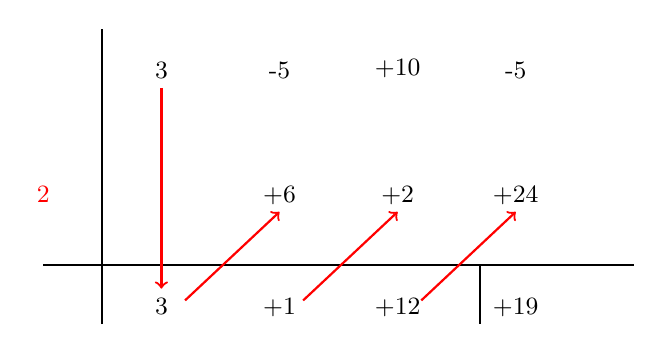
\begin{tikzpicture}[scale=1.5, every node/.style={font=\small}]
    % Draw the axes
    \draw[thick, -] (-0.5, 0) -- (4.5, 0); % Horizontal axis
    \draw[thick, -] (0, -0.5) -- (0, 2); % Vertical axis

    % Top row numbers
    \node[above] at (0.5, 1.5) {3};
    \node[above] at (1.5, 1.5) {-5};
    \node[above] at (2.5, 1.5) {+10};
    \node[above] at (3.5, 1.5) {-5};

    % Bottom row numbers
    \node[below] at (0.5, -0.2) {3};
    \node[below] at (1.5, -0.2) {+1};
    \node[below] at (2.5, -0.2) {+12};
    \node[below] at (3.5, -0.2) {+19};

    % Draw vertical arrow for the first step
    \draw[->, thick, red] (0.5, 1.5) -- (0.5, -0.2);
    \node[below,red] at (-0.5, 0.75) {$2$};

    % Draw horizontal arrows for the transformations
    \draw[->, thick, red] (0.7, -0.3) -- (1.5, 0.45);
    \node[below] at (1.5, 0.75) {+6};

    \draw[->, thick, red] (1.7, -0.3) -- (2.5, 0.45);
    \node[below] at (2.5, 0.75) {+2};

    \draw[->, thick, red] (2.7, -0.3) -- (3.5, 0.45);
    \node[below] at (3.5, 0.75) {+24};
    
    \draw[thick, -] (3.2, 0) -- (3.2, -0.5); % Vertical axis
\end{tikzpicture}

\newpage

\section{Complexe getallen}
\subsection{Rechthoekige coordinaten}
\[
\begin{array}{|l|l|}
\hline
\textbf{Bewerking} & \textbf{Formule} \\ \hline
Optelling/Aftrekking & (a + j.b) \pm (c + j.d) = (a + c) \pm j(b + d) \\ \hline
Vermenigvuldiging & (a + j.b) \cdot (c + j.d) = (ac - bd) + j(ad + bc) \\ \hline
Deling & 
\frac{(a + j.b)}{(c + j.d)} = \frac{(a + j.b) \cdot (c - j.d)}{(c + j.d) \cdot (c - j.d)} = \left( \frac{ac + bd}{c^2 + d^2} \right) + j \left( \frac{bc - ad}{c^2 + d^2} \right) \\ \hline
Toegevoegde\:van & \overline{(a + j.b)} = (a - j.b) \\
& \overline{Z_1 + Z_2} = \overline{Z_1} + \overline{Z_2}, \quad \overline{Z_1 \cdot Z_2} = \overline{Z_1} \cdot \overline{Z_2} \\ \hline
Inverse & z = a + bi \implies z^{-1} = \frac{a - bi}{a^2 + b^2} \\ \hline
Wortel & 
\sqrt{a} \; \wedge \; a < 0 \implies \sqrt{a} = \pm i\sqrt{-a} \\ 
& \sqrt{a + bi} = x + yi \iff (x + yi)^2 = a + bi \\ \hline
Macht & 
(a + bi)^0 = 1 \quad \forall n \in \mathbb{N}_0: \\
& (a + bi)^n = (a + bi) \cdot (a + bi) \cdots (a + bi) \\ \hline
Machten\:of\:i & i^1 = i, \quad i^2 = -1, \quad i^3 = -i, \quad i^4 = 1 \\ \hline
\end{array}
\]

\subsection{Poolcoördinaten}
\[z = a + i.b = r\left( {\cos (\varphi ) + i.\sin (\varphi )} \right) = r\angle \varphi ,\quad \tan (\varphi ) = \frac{b}{a},\quad r = \sqrt {{a^2} + {b^2}} \]
\[
\begin{array}{|l|l|}
\hline
\textbf{Bewerking} & \textbf{Formule} \\
\hline
Vermenigvuldiging & {z_1} \cdot {z_2} = {r_1} \cdot {r_2}\angle {\varphi _1} + {\varphi _2} \\
\hline
Deling & \frac{{{z_1}}}{{{z_2}}} = \frac{{{r_1}\angle {\varphi _1}}}{{{r_2}\angle {\varphi _2}}} = \frac{{{r_1}}}{{{r_2}}}\angle {\varphi _1} - {\varphi _2} \\
\hline
Inverse & {z^{ - 1}} = \frac{1}{r}\angle  - \varphi  \\ \hline
Macht & {z^n} = {r^n}\left[ {\cos \left( {n \cdot \varphi } \right) + i\sin \left( {n \cdot \varphi } \right)} \right]\quad n \in {\displaystyle \mathbb {N} }\\
\hline
Wortel & 
\sqrt {r(\cos \varphi  + i\sin \varphi )}  =  \pm \sqrt r \left( {\cos \frac{\varphi }{2} + i\sin \frac{\varphi }{2}} \right)\\
\hline
\multicolumn{2}{|c|}{\sqrt[n]{{r\left( {\cos \varphi  + i\sin \varphi } \right)}} = \sqrt[n]{r}\left( {\cos \frac{{\varphi  + k \cdot 2\pi }}{n} + i\sin \frac{{\varphi  + k \cdot 2\pi }}{n}} \right)\quad  \wedge \quad k = 0,1, \cdots ,n - 1} \\
\hline
 \end{array}
\]

\newpage

\section{Goniometrie}
\subsection{De Goniometrische Cirkel}

\begin{figure}[h]
\centering
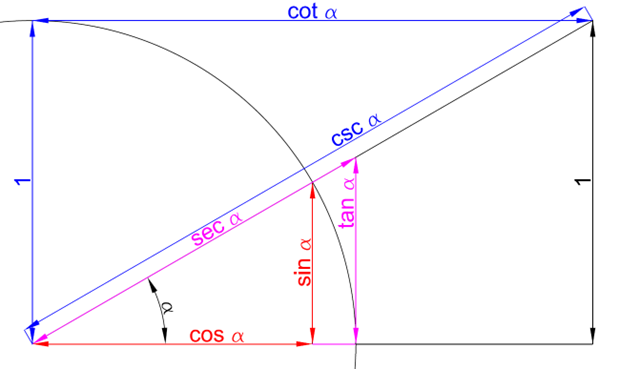
\includegraphics[width=0.8\textwidth]{image_goniometrie.png}
\label{fig:goniometrie}
\end{figure}

\subsection{formules uit de goniometrie}

\begin{figure}[h]
\centering
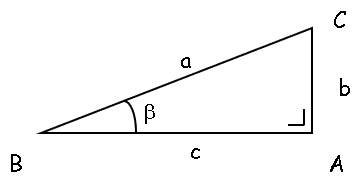
\includegraphics[width=0.4\textwidth]{image_goniometrie_sin_cos_tan.png}
\label{fig:sin_cos_tan}
\end{figure}

{
\[\begin{array}{|c|c|}
\hline
\begin{array}{*{20}{c}}
{\csc \beta }&{sec\beta }&{\cot \beta }\\
 \leftarrow & \leftarrow & \leftarrow \\
{os}&{as}&{oa}\\
 \to & \to & \to \\
{\sin \beta }&{\cos \beta }&{\tan \beta }
\end{array}

& % Scheiding van de twee kolommen

\begin{array}{l}
\text{waarin:} 
\left\{
\begin{aligned}
& o: \text{ overstaande rechthoekszijde} \\
& s: \text{ schuine zijde (hypotenusa)} \\
& a: \text{ aanliggende rechthoekszijde}
\end{aligned}
\right.
\end{array} \\ 
\hline
\end{array}
\]

\[
\begin{array}{|c|c|}
\hline
\text{sin} \, \beta = \frac{b}{a} \hspace{1cm} \text{cos} \, \beta = \frac{c}{a} \hspace{1cm} \text{tan} \, \beta = \frac{b}{c} \\
\hline
\text{csc} \, \beta = \frac{a}{b} \hspace{1cm} \text{sec} \, \beta = \frac{a}{c} \hspace{1cm} \text{cot} \, \beta = \frac{c}{b} \\
\hline
\text{tan} \, \alpha = \frac{\sin \alpha}{\cos \alpha} \hspace{1cm} \text{cot} \, \alpha = \frac{\cos \alpha}{\sin \alpha} \hspace{1cm} \text{cot} \, \alpha = \frac{1}{\tan \alpha} \\
\hline
\text{sec} \, \alpha = \frac{1}{\cos \alpha} \hspace{1cm} \text{csc} \, \alpha = \frac{1}{\sin \alpha}\\
\hline
\end{array}
\]

\[
\boxed{\sin^2{\alpha} + \cos^2{\alpha} = 1} \hspace{1cm}
\boxed{\tan^2{\alpha} + 1 = \sec^2{\alpha}} \hspace{1cm}
\boxed{1 + \cot^2{\alpha} = \csc^2{\alpha}}
\]

\newpage
\begin{figure}
    \centering
    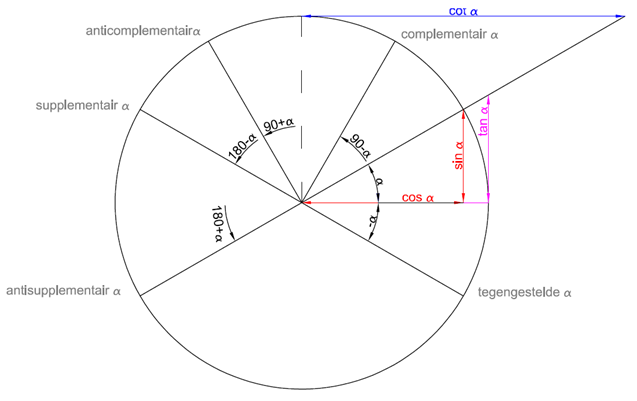
\includegraphics[width=1\linewidth]{image_goniometrie_verwante_hoeken.png}
  
    \label{fig:enter-label}
\end{figure}

\[
\begin{array}{|l|l|l|}
\hline
\text{gelijkehoeken} & \text{supplementairehoeken} & \text{complementairehoeken} \\
\hline
\sin{\left(\alpha + k2\pi\right)} = \sin{\alpha} & \sin{\left(\pi - \alpha\right)} = \sin{\alpha} & \sin{\left(\frac{\pi}{2} - \alpha\right)} = \cos{\alpha} \\
\cos{\left(\alpha + k2\pi\right)} = \cos{\alpha} & \cos{\left(\pi - \alpha\right)} = -\cos{\alpha} & \cos{\left(\frac{\pi}{2} - \alpha\right)} = \sin{\alpha} \\
\tan{\left(\alpha + k2\pi\right)} = \tan{\alpha} & \tan{\left(\pi - \alpha\right)} = -\tan{\alpha} & \tan{\left(\frac{\pi}{2} - \alpha\right)} = \cot{\alpha} \\
\cot{\left(\alpha + k2\pi\right)} = \cot{\alpha} & \cot{\left(\pi - \alpha\right)} = -\cot{\alpha} & \cot{\left(\frac{\pi}{2} - \alpha\right)} = \tan{\alpha} \\
\sec{\left(\alpha + k2\pi\right)} = \sec{\alpha} & \sec{\left(\pi - \alpha\right)} = -\sec{\alpha} & \sec{\left(\frac{\pi}{2} - \alpha\right)} = \csc{\alpha} \\
\csc{\left(\alpha + k2\pi\right)} = \csc{\alpha} & \csc{\left(\pi - \alpha\right)} = \csc{\alpha} & \csc{\left(\frac{\pi}{2} - \alpha\right)} = \sec{\alpha} \\
\hline
\end{array}
\]

\[
\begin{array}{|l|l|l|}
\hline
\text{tegengesteldehoeken} & \text{antisupplementairehoeken} & \text{anticomplementairehoeken} \\
\hline
\sin{\left(-\alpha\right)} = -\sin{\alpha} & \sin{\left(\pi + \alpha\right)} = -\sin{\alpha} & \sin{\left(\frac{\pi}{2} + \alpha\right)} = \cos{\alpha} \\
\cos{\left(-\alpha\right)} = \cos{\alpha} & \cos{\left(\pi + \alpha\right)} = -\cos{\alpha} & \cos{\left(\frac{\pi}{2} + \alpha\right)} = -\sin{\alpha} \\
\tan{\left(-\alpha\right)} = -\tan{\alpha} & \tan{\left(\pi + \alpha\right)} = \tan{\alpha} & \tan{\left(\frac{\pi}{2} + \alpha\right)} = -\cot{\alpha} \\
\cot{\left(-\alpha\right)} = -\cot{\alpha} & \cot{\left(\pi + \alpha\right)} = \cot{\alpha} & \cot{\left(\frac{\pi}{2} + \alpha\right)} = -\tan{\alpha} \\
\sec{\left(-\alpha\right)} = \sec{\alpha} & \sec{\left(\pi + \alpha\right)} = -\sec{\alpha} & \sec{\left(\frac{\pi}{2} + \alpha\right)} = -\csc{\alpha} \\
\csc{\left(-\alpha\right)} = -\csc{\alpha} & \csc{\left(\pi + \alpha\right)} = -\csc{\alpha} & \csc{\left(\frac{\pi}{2} + \alpha\right)} = \sec{\alpha} \\
\hline
\end{array}
\]

\newpage

\begin{table}[H]
    \centering
    \begin{tabular}{|>{\centering\arraybackslash}m{0.4\textwidth}|>{\centering\arraybackslash}m{0.4\textwidth}|}
        \hline
        \begin{minipage}[t]{0.4\textwidth}
            \begin{itemize}
                \item \textbf{De sinusregel:}
                \[
                \frac{a}{\sin \hat{A}} = \frac{b}{\sin \hat{B}} = \frac{c}{\sin \hat{C}}
                \]
                \item \textbf{De cosinusregel:}
                \[
                \begin{aligned}
                    a^2 &= b^2 + c^2 - 2bc\cos \hat{A} \\
                    b^2 &= c^2 + a^2 - 2ca\cos \hat{B} \\
                    c^2 &= a^2 + b^2 - 2ab\cos \hat{C}
                \end{aligned}
                \]
            \end{itemize}
        \end{minipage}
        &
        \begin{minipage}[t]{0.4\textwidth}
            \centering
            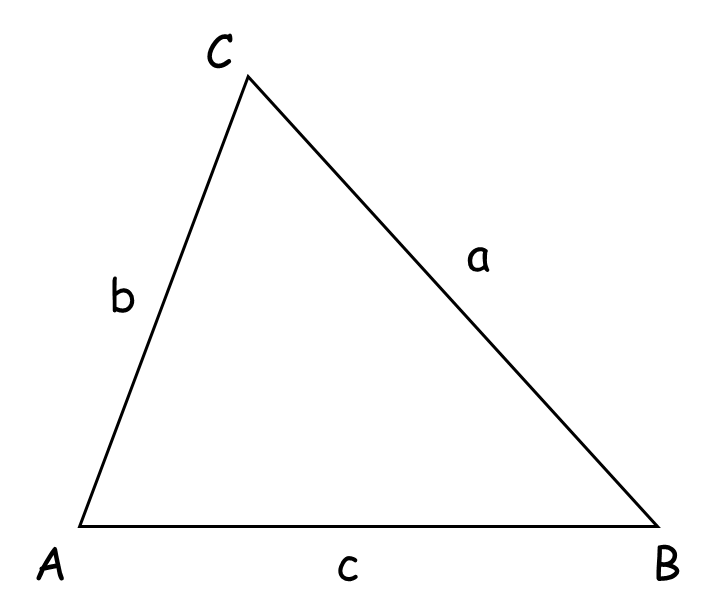
\includegraphics[width=0.9\textwidth]{image_goniometrie_sin_cos_regel.png}
            \label{fig:sin_cos_regel}
        \end{minipage} \\ 
        \hline
    \end{tabular}
\end{table}

\[
\begin{array}{|l|l|}
\hline
\sin(\alpha \pm \beta) = \sin\alpha \cos\beta \pm \cos\alpha \sin\beta & \sin 2\alpha = 2\sin\alpha \cos\alpha \\
\hline
\cos(\alpha \pm \beta) = \cos\alpha \cos\beta \mp \sin\alpha \sin\beta & 
\begin{aligned}
\cos 2\alpha &= \cos^2\alpha - \sin^2\alpha \\
&= 1 - 2\sin^2\alpha \quad (*) \\
&= 2\cos^2\alpha - 1 \quad (**)
\end{aligned} \\
\hline
\tan(\alpha \pm \beta) = \frac{\tan\alpha \pm \tan\beta}{1 \mp \tan\alpha \tan\beta} & 
\tan 2\alpha = \frac{2\tan\alpha}{1 - \tan^2\alpha} \\
\hline
\end{array}
\]

\[
\begin{array}{|l|l|l|}
\hline
\sin^2\alpha = \frac{1 - \cos 2\alpha}{2} \quad (*) & \sin 2\alpha = \frac{2\tan\alpha}{1 + \tan^2\alpha} & 
\sin\alpha = \frac{2t}{1 + t^2} \quad \land \quad \tan\frac{\alpha}{2} = t \\
\cos^2\alpha = \frac{1 + \cos 2\alpha}{2} \quad (**) & \cos 2\alpha = \frac{1 - \tan^2\alpha}{1 + \tan^2\alpha} & 
\cos\alpha = \frac{1 - t^2}{1 + t^2} \\
\sin\frac{\alpha}{2} = \pm\sqrt{\frac{1 - \cos\alpha}{2}} & \tan 2\alpha = \frac{2\tan\alpha}{1 - \tan^2\alpha} & 
\tan\alpha = \frac{2t}{1 - t^2} \\
\cos\frac{\alpha}{2} = \pm\sqrt{\frac{1 + \cos\alpha}{2}} & & \\
\hline
\end{array}
\]
\subsection{Omgekeerde formules van Simpson}
\[
\begin{array}{|c|c|}
\hline
\sin(\alpha \pm \beta) = \sin\alpha\cos\beta \pm \cos\alpha\sin\beta & 
\sin(\alpha + \beta) + \sin(\alpha - \beta) = 2\sin\alpha\cos\beta \\
& 
\sin(\alpha + \beta) - \sin(\alpha - \beta) = 2\cos\alpha\sin\beta \\
\hline
\cos(\alpha \pm \beta) = \cos\alpha\cos\beta \mp \sin\alpha\sin\beta & 
\cos(\alpha + \beta) + \cos(\alpha - \beta) = 2\cos\alpha\cos\beta \\
& 
\cos(\alpha + \beta) - \cos(\alpha - \beta) = -2\sin\alpha\sin\beta \\
\hline
\end{array}
\]
\subsection{Formules van Simpson}
\[
\begin{array}{|c|c|}
\hline
\begin{aligned}
\sin \alpha + \sin \beta &= 2\sin\left(\frac{\alpha + \beta}{2}\right)\cos\left(\frac{\alpha - \beta}{2}\right) \\
\sin \alpha - \sin \beta &= 2\cos\left(\frac{\alpha + \beta}{2}\right)\sin\left(\frac{\alpha - \beta}{2}\right)
\end{aligned} & 
\begin{aligned}
\cos \alpha + \cos \beta &= 2\cos\left(\frac{\alpha + \beta}{2}\right)\cos\left(\frac{\alpha - \beta}{2}\right) \\
\cos \alpha - \cos \beta &= -2\sin\left(\frac{\alpha + \beta}{2}\right)\sin\left(\frac{\alpha - \beta}{2}\right)
\end{aligned} \\
\hline
\end{array}
\]

\newpage
\subsection{Belangrijke goniometrische waarden}
\[
\begin{array}{|c|c|c|c|c|c|c|c|c|c|}
\hline
\text{Angle} & 0^\circ & 30^\circ & 45^\circ & 60^\circ & 90^\circ & 180^\circ & 270^\circ & 360^\circ \\
\hline
\alpha & 0 & \frac{\pi}{6} & \frac{\pi}{4} & \frac{\pi}{3} & \frac{\pi}{2} & \pi & \frac{3\pi}{2} & 2\pi \\
\hline
\sin \alpha & 0 & \frac{1}{2} & \frac{\sqrt{2}}{2} & \frac{\sqrt{3}}{2} & 1 & 0 & -1 & 0 \\
\hline
\cos \alpha & 1 & \frac{\sqrt{3}}{2} & \frac{\sqrt{2}}{2} & \frac{1}{2} & 0 & -1 & 0 & 1 \\
\hline
\tan \alpha & 0 & \frac{1}{\sqrt{3}} & 1 & \sqrt{3} & / & 0 & / & 0 \\
\hline
\end{array}
\]

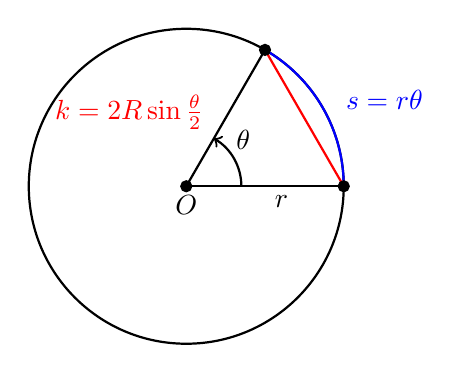
\begin{tikzpicture}

% Draw the circle
\draw[thick] (0,0) circle(2);

% Draw the radius lines
\draw[thick] (0,0) -- (60:2);
\draw[thick] (0,0) -- (0:2);
\draw[thick,red] (60:2) -- (0:2);

% Draw the arc
\draw[thick,blue] (0:2) arc[start angle=0, end angle=60, radius=2];

% Add the center point O
\filldraw[black] (0,0) circle(2pt) node[below] {\( O \)};

% Add the point on the arc
\filldraw[black] (60:2) circle(2pt);
\filldraw[black] (0:2) circle(2pt);

% Add labels
\node[below right] at (0:1) {\( r \)};
\node[right,blue] at (30:2.2) {\( s = r\theta \)};
\node[left,red ] at (70:1) {$k = 2R \sin\frac{\theta}{2}$};
\node[above] at (25:0.8) {\( \theta \)};

% Draw the angle
\draw[thick,->] (0:0.7) arc[start angle=0, end angle=60, radius=0.7];

\end{tikzpicture}

\subsection{Cyclometrische formules}

\[\begin{array}{*{20}{l}}
{y = {\mathop{\rm Bgsin}\nolimits} x \Leftrightarrow \left( {x = \sin y\;\; \wedge y \in \left[ { - \frac{\pi }{2},\frac{\pi }{2}} \right],\;x \in \left[ { - 1,1} \right]} \right)}\\
{y = {\mathop{\rm Bgcos}\nolimits} x \Leftrightarrow \left( {x = \cos y\;\; \wedge y \in \left[ {0,\pi } \right],\;x \in \left[ { - 1,1} \right]} \right)}\\
{y = {\mathop{\rm Bgtan}\nolimits} \;x \Leftrightarrow \left( {x = \tan y\;\; \wedge y \in \left] { - \frac{\pi }{2},\frac{\pi }{2}} \right[,\;x \in \mathbb {R} } \right)}
\end{array}\]

\begin{figure}[h!]
    \centering
    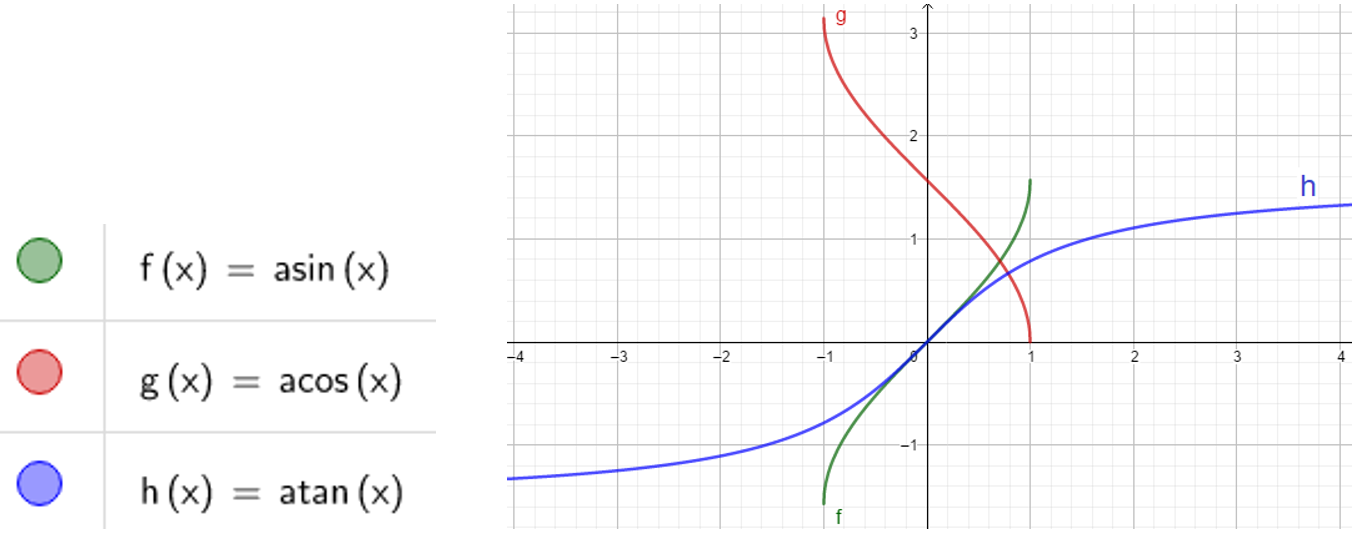
\includegraphics[width=0.6\linewidth]{image_goniometrie_cyclof.png}
    \label{fig:enter-label}
\end{figure}

\[\begin{array}{*{20}{c}}
{\sin \left( {{\mathop{\rm Bgsin}\nolimits} x} \right) = x \wedge \forall x \in \left[ { - 1,1} \right]}&{\cos \left( {{\mathop{\rm Bgtan}\nolimits} x} \right) = \frac{1}{{\sqrt {1 + {x^2}} }}\forall x \in \mathbb {R} }\\
{\cos \left( {{\mathop{\rm Bgcos}\nolimits} x} \right) = x \wedge \forall x \in \left[ { - 1,1} \right]}&{\sin \left( {{\mathop{\rm Bgtan}\nolimits} x} \right) = \frac{x}{{\sqrt {1 + {x^2}} }}\forall x \in \mathbb {R} }\\
{tg\left( {{\mathop{\rm Bgtan}\nolimits} } \right) = x \wedge \forall x \in \mathbb {R} }&{{\mathop{\rm Bgsin}\nolimits} x + {\mathop{\rm Bgcos}\nolimits} x = \frac{\pi }{2} \wedge \forall x \in \left[ { - 1,1} \right]}\\
{cotg\left( {{\mathop{\rm Bgcot}\nolimits} x} \right) = x \wedge \forall x \in \mathbb {R} }&{{\mathop{\rm Bgcot}\nolimits} x + {\mathop{\rm Bgtan}\nolimits} x = \frac{\pi }{2} \wedge \forall x \in \mathbb {R} }\\
{\cos \left( {{\mathop{\rm Bgsin}\nolimits} x} \right) = \sqrt {1 - {x^2}} \wedge \forall x \in \left[ { - 1,1} \right]}&{{\mathop{\rm Bgtan}\nolimits} \left( { - x} \right) =  - {\mathop{\rm Bgtan}\nolimits} x \wedge \forall x \in \mathbb {R} }\\
{\sin \left( {{\mathop{\rm Bgcos}\nolimits} x} \right) = \sqrt {1 - {x^2}}  \wedge\forall x \in \left[ { - 1,1} \right]}&{{\mathop{\rm Bgcot}\nolimits} \left( { - x} \right) =  - {\mathop{\rm Bgcot}\nolimits} x \wedge \forall x \in \mathbb {R} }\\
{Bgsin\left( { - x} \right) =  - {\mathop{\rm Bgsin}\nolimits} x \wedge \forall x \in \left[ { - 1,1} \right]}&{{\mathop{\rm Bgcos}\nolimits} \left( { - x} \right) = \pi  - {\mathop{\rm Bgcos}\nolimits} x\forall x \in \left[ { - 1,1} \right]}
\end{array}\]

\newpage

\section{Meetkunde}

$
\begin{array}{|l|l|}
\hline
\text{Afstand 2 punten} & \left| {{P_1}({x_1},{y_1}),{P_2}({x_2},{y_2})} \right| = \sqrt {{{({x_2} - {x_1})}^2} + {{({y_2} - {y_1})}^2}}  \\
 & \begin{array}{l}
\left| {{P_1}({x_1},{y_1},{z_1}),{P_2}({x_2},{y_2},{z_2})} \right| = \\
\sqrt {{{({x_2} - {x_1})}^2} + {{({y_2} - {y_1})}^2} + {{({z_2} - {z_1})}^2}} 
\end{array} \\
\hline
\text{Midden v/e lijnstuk} & co(M) = (\frac{{({x_1} + {x_2})}}{2},\frac{{({y_1} + {y_2})}}{2})\\
\hline
\text{Zwaartepunt v/e driehoek} & co(Z) = (\frac{{({x_1} + {x_2} + {x_3})}}{3},\frac{{({y_1} + {y_2} + {y_3})}}{3})\\
\hline
\end{array}
$
\newline
$
\begin{array}{|l|l|}
\hline
\text{Vergelijking v/e rechte dr punt met rico m} & y - {y_1} = m(x - {x_1})  \\
\hline
\text{Vergelijking v/e rechte dr punt met rico m} & y - {y_1} = \frac{{{y_2} - {y_1}}}{{{x_2} - {x_1}}}(x - {x_1})  \\
\hline
\text{Vergelijking v/e rechte dr snijpunt met x-as (r,0) en y-as (0,s)} & \frac{x}{r} + \frac{y}{s} = 1  \\
\hline
\text{Hoek tussen twee rechten a,b met rico m1,m2} & \cos (\widehat {ab}) = \frac{{\left| {1 + {m_1}{m_2}} \right|}}{{\sqrt {1 + {m_1}^2} \sqrt {1 + {m_2}^2} }}  \\
\hline
\text{Afstand tussen rechte a->ux+vy+w=0 en P(x1,y1)} & d(P,a) = \frac{{\left| {u{x_1} + v{y_1} + w} \right|}}{{\sqrt {{u^2} + {v^2}} }}  \\
\hline
\end{array}
$

\subsection{De cirkel}

$
\begin{array}{|l|l|}
\hline
\text{Cartesiaanse vergelijking} & {(x - {x_1})^2} + {(y - {y_1})^2} = {r^2}  \\
\hline
\text{Algemene vergelijking} & {x^2} + {y^2} + 2ax + 2by + c = 0\quad  \wedge \quad {a^2} + {b^2} - c \ge 0  \\
\hline
\text{Parameter vergelijking} & \left\{ {\begin{array}{*{20}{c}}
{x = {x_M} + r.\cos t}\\
{y = {y_M} + r.\sin t}
\end{array}} \right.\;\quad \quad met\;t \in \left[ {0,2\pi } \right[  \\
\hline
\end{array}
$

\subsection{De parabool}

$
\begin{array}{|l|l|}
\hline
\text{Top vergelijking} & {y^2} = 2px  \\
\hline
\text{Parameter vergelijking} & \begin{array}{l}
x = 2p{\lambda ^2}\quad \quad met\;\lambda  \in \mathbb {R} \\
y = 2p\lambda 
\end{array}  \\
\hline
\end{array}
$

\newpage

\section{Diversen}
\subsection{Wiskundige Symbolen (ISO 31/XI)}
$
\begin{array}{|l|l|}
\hline
x \in A & \text{is een element van de verzameling} \\
x \not\in A & \text{is geen element van de verzameling} \\
\{x_1, x_2, \dots, x_n\} & \text{de verzameling door opsomming} \\
\{ x \in \left. A \right|p(x)\} & \text{de verzameling waar de elementen voldoen aan de eigenschap } p(x) \\
\hline
\emptyset & \text{de lege verzameling} \\
\mathbb{N} & \text{de natuurlijke getallen } (0,1,2,\dots) \\
\mathbb{Z} & \text{de gehele getallen } (\dots, -2,-1,0,1,2,\dots) \\
\mathbb{Q} & \text{de rationale getallen (breuken van } \mathbb{Z} \text{)} \\
\mathbb{R} & \text{de reële getallen} \\
\mathbb{C} & \text{de complexe getallen} \\
\hline
B \subseteq A & B \text{ behoort tot } A \text{ (kan er mee samenvallen)} \\
B \subset A & B \text{ behoort strikt tot } A \\
A \cup B & \text{samenvoeging van } A \text{ en } B \text{ (unie)} \\
A \cap B & \text{doorsnede van } A \text{ en } B \text{ (de gemeenschappelijke elementen)} \\
A \setminus B & A \text{ verschilt } B \text{, wat tot } A \text{ behoort en niet tot } B \\
\mathcal{C}_U A & \text{het complement van } A \text{ in het universum } U \\
\hline
(a,b) & \text{het geordend paar} \\
(a_1, a_2, \dots, a_n) & \text{een geordend } n \text{-tal} \\
A \times B & \text{de productverzameling van } A \text{ en } B \\
\# & \text{rangnummer of aantal} \\
\hline
\end{array}
$
\subsection{Logische symbolen}
$
\begin{array}{|l|l|}
\hline
p \land q & \text{conjunctie, de beweringen } p \text{ en } q \text{ zijn geldig} \\
p \lor q & \text{disjunctie, de bewering } p \text{ of } q \text{ is geldig} \\
\lnot p & \text{negatie, de bewering } p \text{ is niet geldig} \\
p \Rightarrow q & \text{implicatie, als } p \text{ dan } q \\
p \Leftrightarrow q & \text{equivalentie, de beweringen } p \text{ en } q \text{ zijn gelijkwaardig} \\
\forall x & \text{universele kwantor, voor alle elementen geldt} \\
\exists x & \text{existentiële kwantor, er zijn elementen die voldoen aan} \\
\hline
\end{array}
$
\end{document}
